% ================================================================
% CHAPTER 6: Anhang: Dokumentation
% ================================================================
\section{Dokumentation zum entwickelten System }
\subsection{Computer für Entwicklung}
\subsubsection{Basisinformationen}
\begin{table}[H]
	\rowcolors{2}{maroon!10}{white!100}
	\arrayrulecolor{darkmaroon} 
	
	\begin{tabular}{p{6cm} p{8cm}}
		
		\toprule[1pt]
		\rowcolor{maroon!30}
		
		Begriff & Spezifikation\\
		
		\midrule 
		Modell & Mac mini (Late 2014) \\
		Betriebssystem & macOS Catalina Version 10.15.3\\
		Prozessor & 2.6 GHz Dual-Core Intel Core i5\\
		Speicher &  8 GB 1600 MHz DDR3\\
		Grafikkarte & Intel Iris 1536 MB\\
		Seriennummer & C07QG49TG1HW\\
		
		\bottomrule
	\end{tabular}
	\caption{Basisinformationen zum Computer Entwicklung}
	\label{fig: Basisinformationen zum Computer Entwicklung}
\end{table}

\subsection{Eingesetzte Software}
Nachfolgend wird die wertschöpfende Software mit dem entsprechenden Verwendungszweck und der eingesetzen Version genannt.
\begin{table}[H]
	\rowcolors{2}{maroon!10}{white!100}
	\arrayrulecolor{darkmaroon} 
	
	\begin{tabular}{p{3cm} p{8cm} p{3cm} }
		
		\toprule[1pt]
		\rowcolor{maroon!30}
		
		Software & Verwendungszweck & Version\\
		
		\midrule 
		Python  & Programmiersprache für Housekeeping und Auslösung der spezfischen Aktionen ausgehend vom Erreichen oder Nichterreichen der merkmalsbezogenen Schwellwertes & 3.7.4\\
		OpenCV &  Programmbibliothek mit Algorithmen für die Bildverarbeitung und maschinelles Sehen & 4.2.0 \\ 		

		\bottomrule
	\end{tabular}
	\caption{Eingesetzte Software Entwicklung}
	\label{fig: Eingesetzte Software Entwicklung}
\end{table}

\subsection{Installation von OpenCV und vorausgesetzten Softwaremodulen}

\subsubsection{Xcode installieren und Lizenzvereinbarung akzeptieren} 
\begin{itemize}
	\item Im App Store anmelden und Xcode herunterladen
	\item \texttt{sudo xcodebuild -license}
	\item \texttt{sudo xcode-select --install}
\end{itemize}

\subsubsection{Apple Command Line Tools installieren} 
\begin{itemize}
	\item \texttt{sudo xcode-select --install}
\end{itemize}

\subsubsection{Homebrew installieren und Bash Profil anpassen} 
\begin{itemize}
	\item \texttt{/usr/bin/ruby -e \grqq\$(curl -fsSL \newline https://raw.githubusercontent.com/Homebrew/install/master/install)\grqq}
	\item \texttt{brew update}
	\item \texttt{echo \grqq\# Homebrew\grqq  $>$$>$ \textasciitilde/.bash\_profile}
	\item \texttt{echo \grqq export PATH=/usr/local/bin:\$PATH \grqq >> \textasciitilde/.bash\_profile}

\end{itemize}


\subsubsection{Pakete installieren} 
\begin{itemize}
	\item \texttt{brew install cmake pkg-config}
	\item \texttt{brew install qt5}
	\item \texttt{brew install wget}
	
\end{itemize}

\subsubsection{Konfiguration und Ordnerstruktur vorbereiten } 
\begin{itemize}
	\item \texttt{QT5PATH=/usr/local/Cellar/qt/5.14.1}
	\item \texttt{cwd=\$(pwd)}
	\item \texttt{cvVersion=\grqq master\grqq}
	
	\item \texttt{rm -rf opencv/build}	
	\item \texttt{rm -rf opencv\_contrib/build}
	\item \texttt{mkdir installation}
	\item \texttt{mkdir installation/OpenCV-\grqq\$cvVersion\grqq}	
	
\end{itemize}

\subsubsection{Python Pakete installieren und virtuelle Umgebung einrichten } 
\begin{itemize}
	\item \texttt{sudo -H pip3 install -U pip numpy}
	\item \texttt{sudo -H python3 -m pip install virtualenv virtualenvwrapper}
	\item \texttt{VIRTUALENVWRAPPER\_PYTHON=/usr/local/bin/python3}
	\item \texttt{echo \grqq VIRTUALENVWRAPPER\_PYTHON=/usr/local/bin/python3\grqq  $>$$>$ \newline ~/.bash\_profile}
	\item \texttt{	echo \grqq \# Virtual Environment Wrapper\grqq $>$$>$ ~/.bash\_profile}
	\item \texttt{ 	echo \grqq source /usr/local/bin/virtualenvwrapper.sh\grqq $>$$>$ ~/.bash\_profile }
	\item \texttt{mkvirtualenv OpenCV-\grqq\$cvVersion\grqq-py3 -p python3}	
	\item \texttt{workon OpenCV-\grqq\$cvVersion\grqq -py3s	}
	\item \texttt{pip install cmake numpy scipy matplotlib scikit-image scikit-learn ipython dlib}
	\item \texttt{deactivate}	
\end{itemize}

\subsubsection{GitHub Repositories klonen } 
\begin{itemize}
	\item \texttt{git clone https://github.com/opencv/opencv.git}
	\item \texttt{cd opencv}	
	\item \texttt{git checkout master}	
	\item \texttt{cd ..}
	\item \texttt{git clone https://github.com/opencv/opencv\_contrib.git}
	\item \texttt{cd opencv\_contrib}	
	\item \texttt{git checkout master}	
	\item \texttt{cd ..}
	\item \texttt{cd opencv}
	\item \texttt{mkdir build}	
	\item \texttt{cd build}	
	
\end{itemize}

\subsubsection{Build erstellen} 
\texttt{
	cmake -D CMAKE\_BUILD\_TYPE=RELEASE \textbackslash \newline 
	-D CMAKE\_INSTALL\_PREFIX=\$cwd/installation/OpenCV-\grqq\$cvVersion \grqq \textbackslash \newline
	-D INSTALL\_C\_EXAMPLES=OFF \textbackslash \newline
	-D INSTALL\_PYTHON\_EXAMPLES=ON \textbackslash \newline
	-D WITH\_TBB=ON \textbackslash \newline
	-D WITH\_V4L=ON \textbackslash \newline
	-D OPENCV\_SKIP\_PYTHON\_LOADER=ON \textbackslash \newline
	-D CMAKE\_PREFIX\_PATH=\$QT5PATH \textbackslash \newline
	-D CMAKE\_MODULE\_PATH=\grqq\$QT5PATH\grqq/lib/cmake \textbackslash \newline
	-D OPENCV\_PYTHON3\_INSTALL\_PATH=\textasciitilde/.virtualenvs/OpenCV-\grqq\$cvVersion\grqq-py3/lib/python3.7/site-packages \textbackslash \newline
	-D WITH\_QT=ON \textbackslash \newline
	-D WITH\_OPENGL=ON \textbackslash \newline
	-D OPENCV\_EXTRA\_MODULES\_PATH=../../opencv\_contrib/modules \textbackslash \newline
	-D BUILD\_EXAMPLES=ON  \newline
}	

\subsubsection{OpenCV 4 kompilieren}
\begin{itemize}
 	\item \texttt{make -j\$(sysctl -n hw.physicalcpu)}
  	\item \texttt{make install}
 	\item \texttt{cd \$cwd} 	
\end{itemize}


\subsubsection{Spyder für die Benützung mit der virtuellen Umgebung einrichten}
\begin{itemize}
	\item \texttt{workon OpenCV-master-py3}	
	\item \texttt{pip install spyder-kernels==0.*}	
	\item \texttt{python -c \grqq import sys; print(sys.executable)\grqq}: 
	\item Die Ausgabe dieses Befehls in den Zwischenspeicher kopieren. \item Spyder öffnen und in den Voreinstellungen den Menupunkt \grqq Python-Interpreter\grqq{} wählen. 
	\item Den Inhalt aus dem Zwischenspeicher als Pfad zum Python-Interpreter verwenden.
\end{itemize}


\subsection{Nützliche Links}

\begin{table}[H]
	\rowcolors{2}{maroon!10}{white!100}
	\arrayrulecolor{darkmaroon} 
	
	\begin{tabular}{p{6cm} p{9cm}|}
		
		\toprule[1pt]
		\rowcolor{maroon!30}
		
		Stichwort & URL \\
		
		\midrule 	
		Informationen zu OpenCV & \url{opencv.org}\\
		OpenCV-Python Tutorials und Dokumentation & \url{opencv-python-tutroals.readthedocs.io/en/latest}\\

		
		\bottomrule
	\end{tabular}
	\caption{Nützliche Links}
	\label{fig: Nützliche Links}
\end{table}

\begin{landscape}
\section{Mindmap als Entwurf für Modellierung der Domäne}
\begin{figure}[H]
	\center
	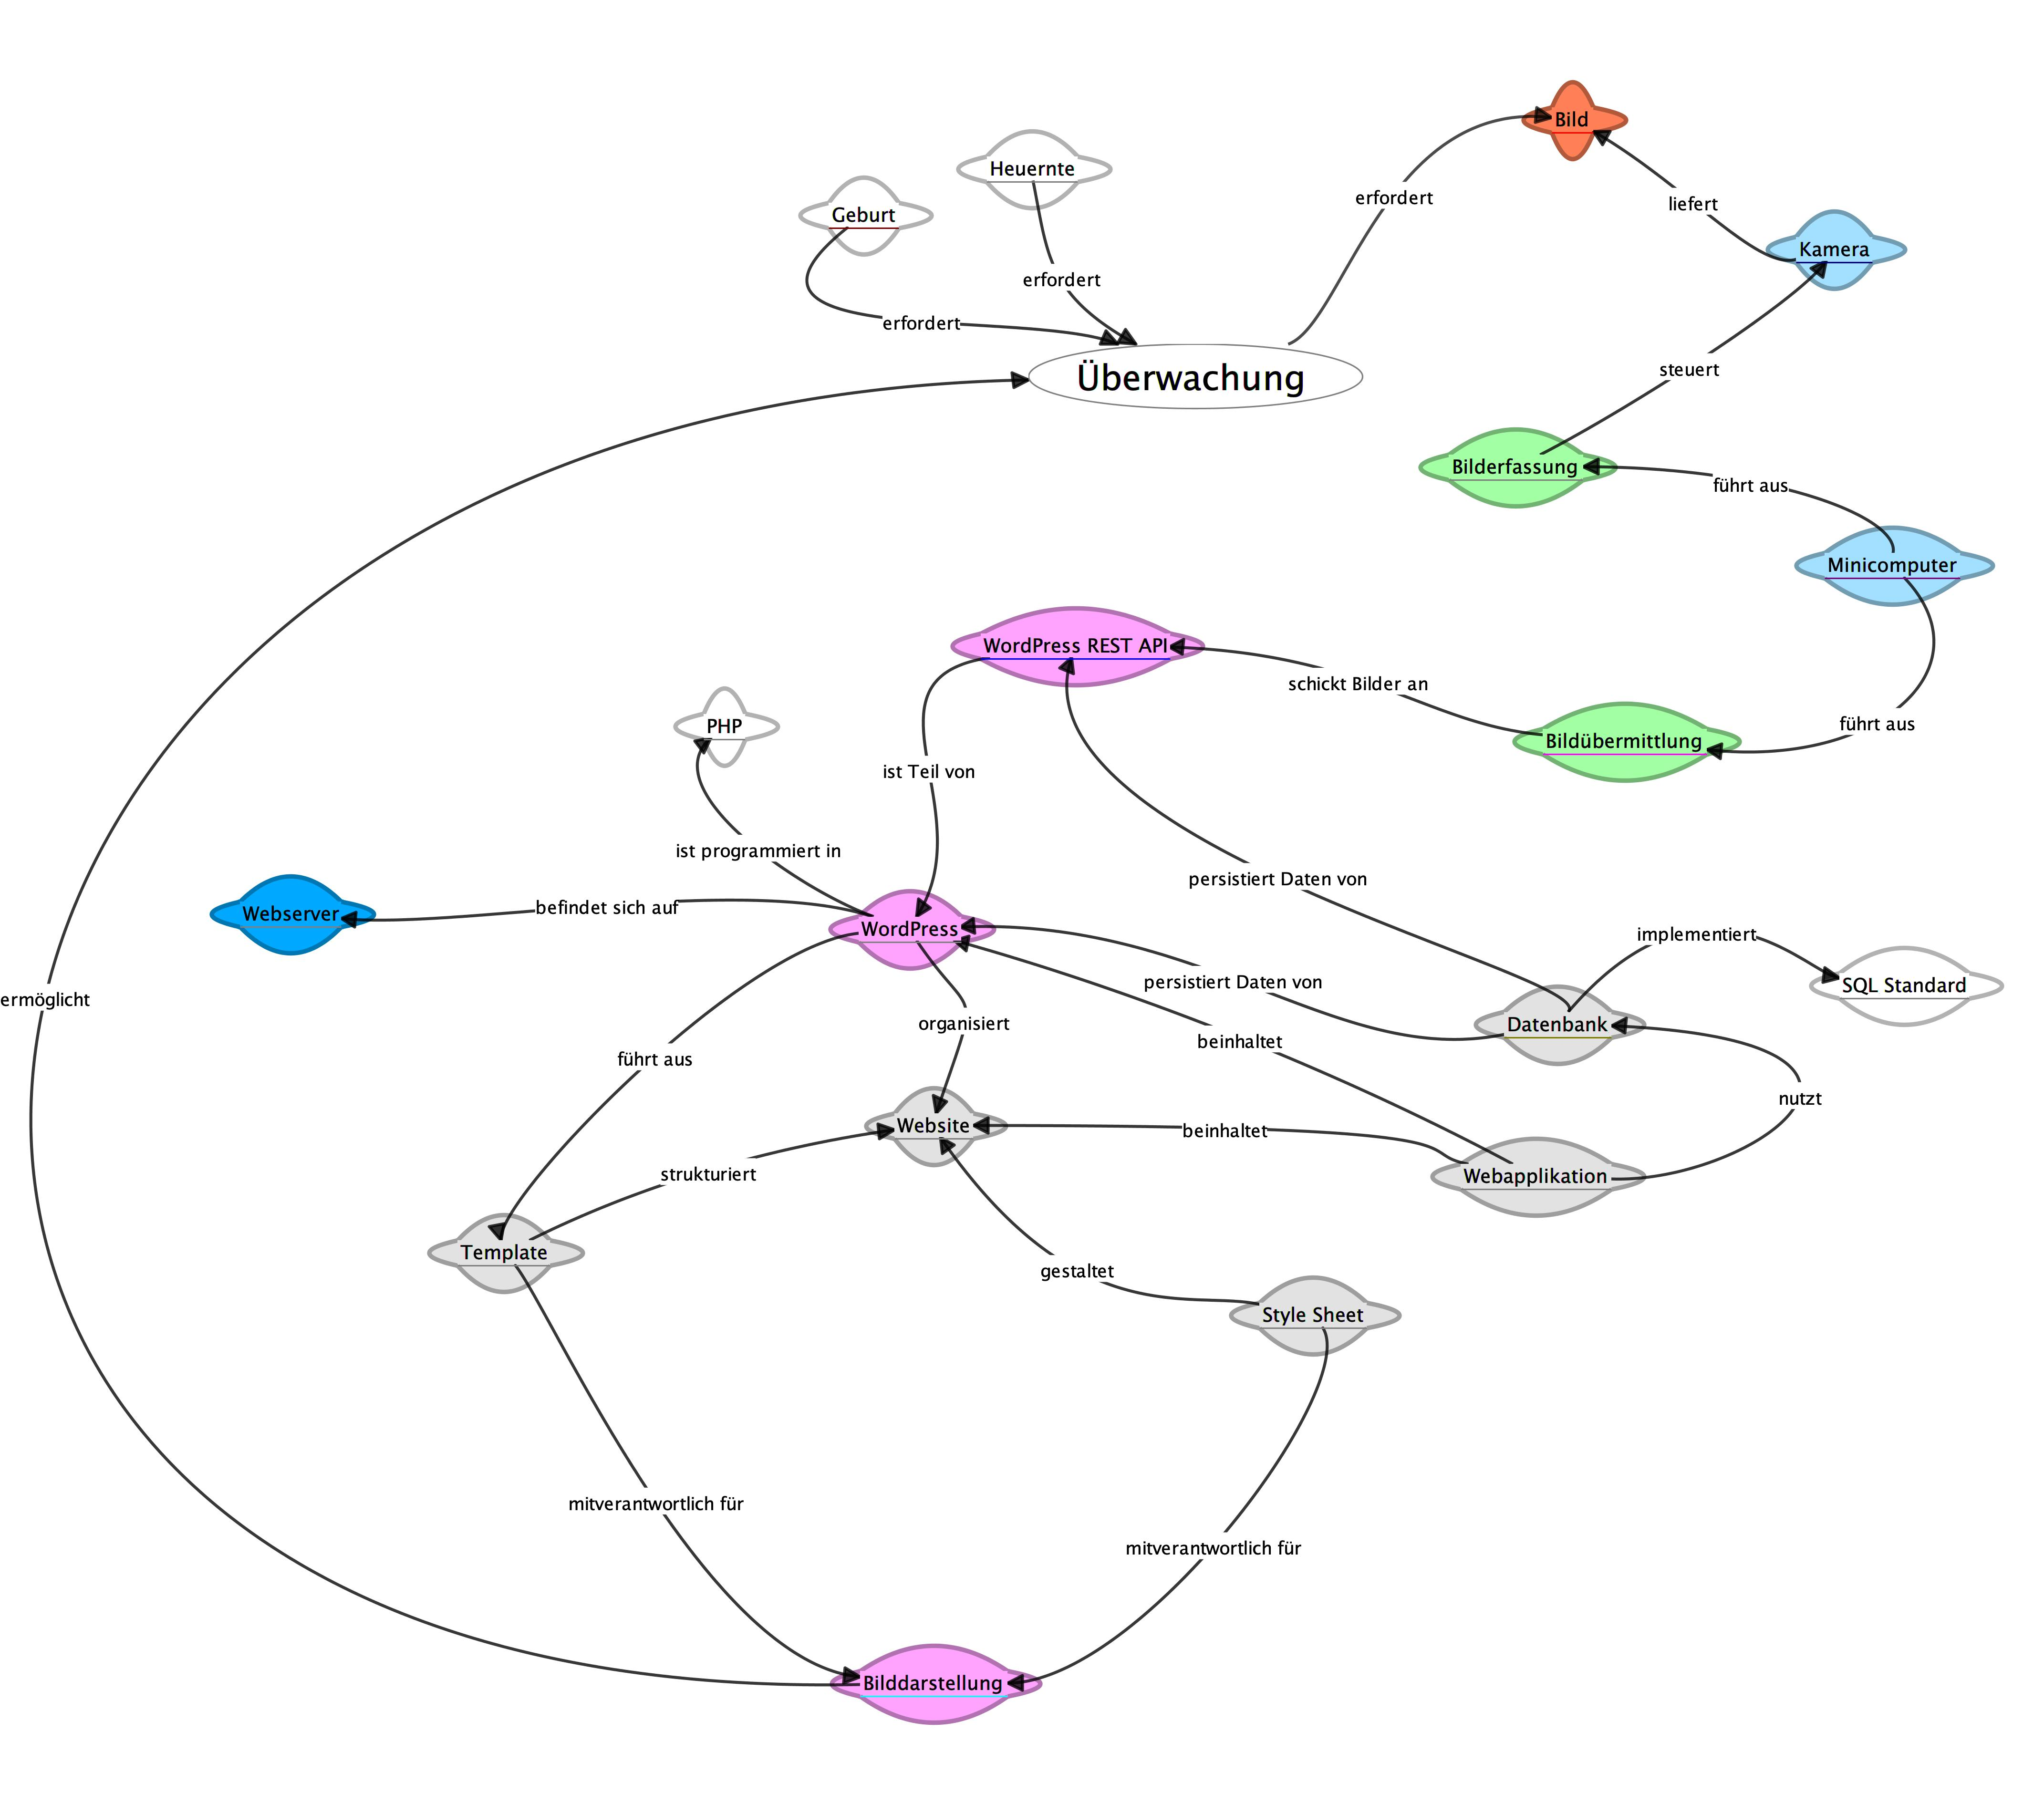
\includegraphics[scale=.09]{Grafiken/mmDomain.jpg}
	\caption{Mindmap als Entwurf für die Modellierung der Domäne. Farbcodierung gemäss Tabelle }
	\label{fig: Mindmap als Entwurf die für Modellierung der Domäne. Farbcodierung gemäss Tabelle}
\end{figure}
	
\end{landscape}